\documentclass[11pt]{article}
\usepackage{amsmath, amssymb, amsthm}
\usepackage{fullpage}
\usepackage{tikz}
\usetikzlibrary{shapes.geometric}
\usetikzlibrary{arrows}
\usepackage{amsmath}
\usepackage{hyperref}

\newcounter{excounter}
\setcounter{excounter}{1}
\newcommand\question[2]{\vskip 1em  \noindent\textbf{\arabic{excounter}\addtocounter{excounter}{1}:} (\emph{#1}) \newline \noindent#2}
\newcommand\hint[1]{ \newline \noindent\textit{Hint: #1}}
\newcommand\solution[1]{\vskip 0.5em \noindent\textbf{Solution:}\par\noindent#1}

\renewcommand\solution[1]{ }



\begin{document}
\large

{\bf MATH-566 \hspace{1cm} HW 10}
\vskip 1em
Due \textbf{Dec 9} before class (regularly). Just bring it before the class and it will be collected there.

Complete 5 questions.


\question{Branch and bound}{
Solve the following problem using branch and bound. Draw the branching tree too.
\[
(P)=\begin{cases}
\text{maximize} & -x_1 + 4x_2\\
\text{subject to} & -10x_1 + 20x_2 \leq 22 \\
                          &   5x_1 +10x_2 \leq 49 \\ 
                          &  x_1 \leq 5\\
                          & x_i \geq 0,  x_i \in \mathbb{Z} \text{ for } i \in \{1,2\}
\end{cases}                          
\]
You can use any linear programming solver for solving the relaxations.
}


\question{Cutting planes}{
Let $P$ be a convex hull of $(0,0), (0,1), (k,\frac{1}{2})$. Give an upper bound on Chv\'atal's rank of $P$. (Show it is at most $2k$, actually, it is exactly $2k$.)\\
\emph{Hints: Write $P$ as an intersection of half-spaces, use \emph{induction} on  $k$. See what we were doing in notes.}\\
Drawing of $P$  for $k=3$.
\begin{center}
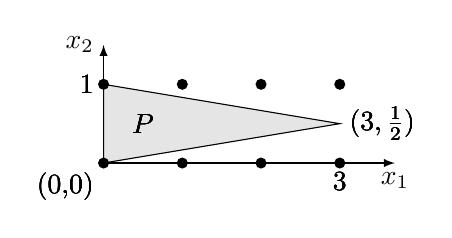
\begin{tikzpicture}[scale=1]
\draw[fill=gray!20]
(0,0) -- (3,0.5) -- (0,1) -- cycle
;
\foreach \x in {0,1,2,3}{
\foreach \y in {0,1}{
\fill (\x,\y) circle(2 pt);
}
\draw
(0,0) node[below left]{(0,0)}
(0,1) node[left]{1}
(3,0) node[below]{3}
(3,0.5) node[right]{$(3,\frac{1}{2})$}
;
\draw
(0.5,0.5) node{$P$}
;
}
\draw[-latex](0,0) -- (3.7,0) node[below]{$x_1$};
\draw[-latex](0,0) -- (0,1.5) node[left]{$x_2$};
\end{tikzpicture}
\end{center}
}



\question{Can you do Edmonds?}{
Run Edmond's Blossom algorithm on the following graph. Notice that somebody
already found a partial matching. What is the largest possible matching?
Try to start growing augmenting tree from $x$, use BFS algorithm for building the tree.
\begin{center}
\tikzset{insep/.style={inner sep=2.2pt, outer sep=0pt, circle, fill},}
\begin{tikzpicture}[scale=1.5]
\draw   
(0,0) node[insep,label=left: ](a){} 
(1,0) node[insep,label=left: ](b){}
++(72:1) node[insep,label=left: ](c){}
++(144:1) node[insep,label=left: ](d){}
++(216:1) node[insep,label=left: ](e){}
(b) ++ (-72:1) node[insep,label=left: ](g){}  
++(-144:1) node[insep,label=left: ](i){}
++(-216:1) node[insep,label=left: ](j){}
(c) ++(1,0) node[insep,label=left: ](f){} 
(g) ++(1,0) node[insep,label=left: ](h){} 
(d) ++ (3,0) node[insep,label=left: ](k){}
(i) ++ (3,0) node[insep,label=left: ](l){}
(b) ++ (3.5,0) node[insep,label=left: ](m){}
(d) ++ (-3,0) node[insep,label=left: ](n){}
(i) ++ (-3,0) node[insep,label=left: ](o){}
(a) ++ (-3.5,0) node[insep,label=left:$x$](p){}
;
\draw
(a)--(b) (a)--(e) (a)--(j) (b)--(g)--(h) (g)--(i)
(n)--(d)--(k)--(m)--(l)--(i)--(o)--(p)--(n) (n)--(o)
(d)--(c)--(f) (k)--(l)
;
\draw[line width=2.5pt]
(n)--(o) (e)--(d) (i)--(j) (b)--(c) (f)--(h) 
;
\draw[dashed]
;
\end{tikzpicture}
\end{center}
}


\question{Can you do weighted bipartite matching?}{
Find minimum-weight perfect matching in the following graph:
\begin{center}
\tikzset{insep/.style={inner sep=1.5pt, outer sep=0pt, circle, fill},}
\begin{tikzpicture}[scale=1.5]
\draw   (0,0) node[insep,label=left:$x$](r){} 
++(45:1)  node[insep,label=above: ](a){}
++(0:1)  node[insep,label=above: ](b){}
(r) ++(-45:1)  node[insep,label=below: ](d){}
++(0:1)  node[insep,label=below: ](f){}
++(45:1) node[insep,label=above: ](g){}
++(0:1) node[insep,label=above: ](h){}
(f) ++(0:1.5) node[insep,label=below: ](i){}
;
\draw
(r) -- node[above]{1} (a)
(r) -- node[below]{4} (d)
(a) -- node[above]{4} (b)
(d) -- node[above]{2} (f)
(g) -- node[above]{4} (h)
(b) -- node[above]{5} (g)
(f) -- node[above]{4} (g)
(f) -- node[above]{6} (i)
(h) -- node[right]{3} (i)
;
\end{tikzpicture}
\end{center}
A) By using algorithm from class that grows augmenting tree (and keep primal/dual solutions). Start growing $x$.\\
B) Formulate the problem using Integer/Linear programming and solve it with your favorite solver.
}



\question{Understanding maximum matching}{
Slither is a two-person game played on a graph $G=(V,E)$. 
The players, called First and Second, play alternatively, with First playing first.
At each step the player whose turn it is chooses a previously unchosen edge.
The only rule is that at every step the set of chosen edges forms a path.
The loser is the first player unable to make a legal move at his or her turn.
Prove that if $G$ has a perfect matching, then First can force a win.
}


\question{Programming A}{Implement algorithm for finding maximum matching in bipartite graphs.
Test it on the 3D-cube.
}

\question{Programming B}{Implement algorithm for finding maximum matching in any graph.\\
Test it on the 3D-cube and the graph from question 3.\\
(Doing this will also solve the previous question - 2 for 1.)
}


\end{document}
